% \setchapterpreamble[u]{\margintoc}
\chapter{Networking and SSH}
\labch{ssh}


\section{Networking}

\subsection{What is networking?}

Have you ever tried to get some work done on a computer
while the internet was down? It's a nightmare.
Modern day computing relies highly on networking.
But what is networking?

\begin{definition}[Networking]
A computer network comprises two or more computers
that are connected—either by cables (wired) or wifi
(wireless)—with the purpose of transmitting, exchanging,
or sharing data and resources.
\end{definition}

We have been using the computer, and linux, for a while now
but the utility of a computer increases exponentially when
it is connected to a network. It allows computers to share
files and resources, and to communicate with each other.
Current day world wide web is built on the internet.

\begin{definition}[Internet]
Internet is a global network of networks that connects
millions of computers worldwide. It allows computers to
connect to other computers across the world through a
hierarchy of routers and servers.
\end{definition}

Learning about networking and how networking works
is useful, although we won't be devling into details
in this book. It is left as an exercise for the reader
to explore external resources if they are interested.

\marginnote{
One succinct blogpost explaining how the internet works
from which the figure \reffig{networks} is taken
is available at
\url{https://www.highspeedinternet.com/resources/how-the-internet-works}
}

\subsection{Types of Networks}

\begin{marginfigure}
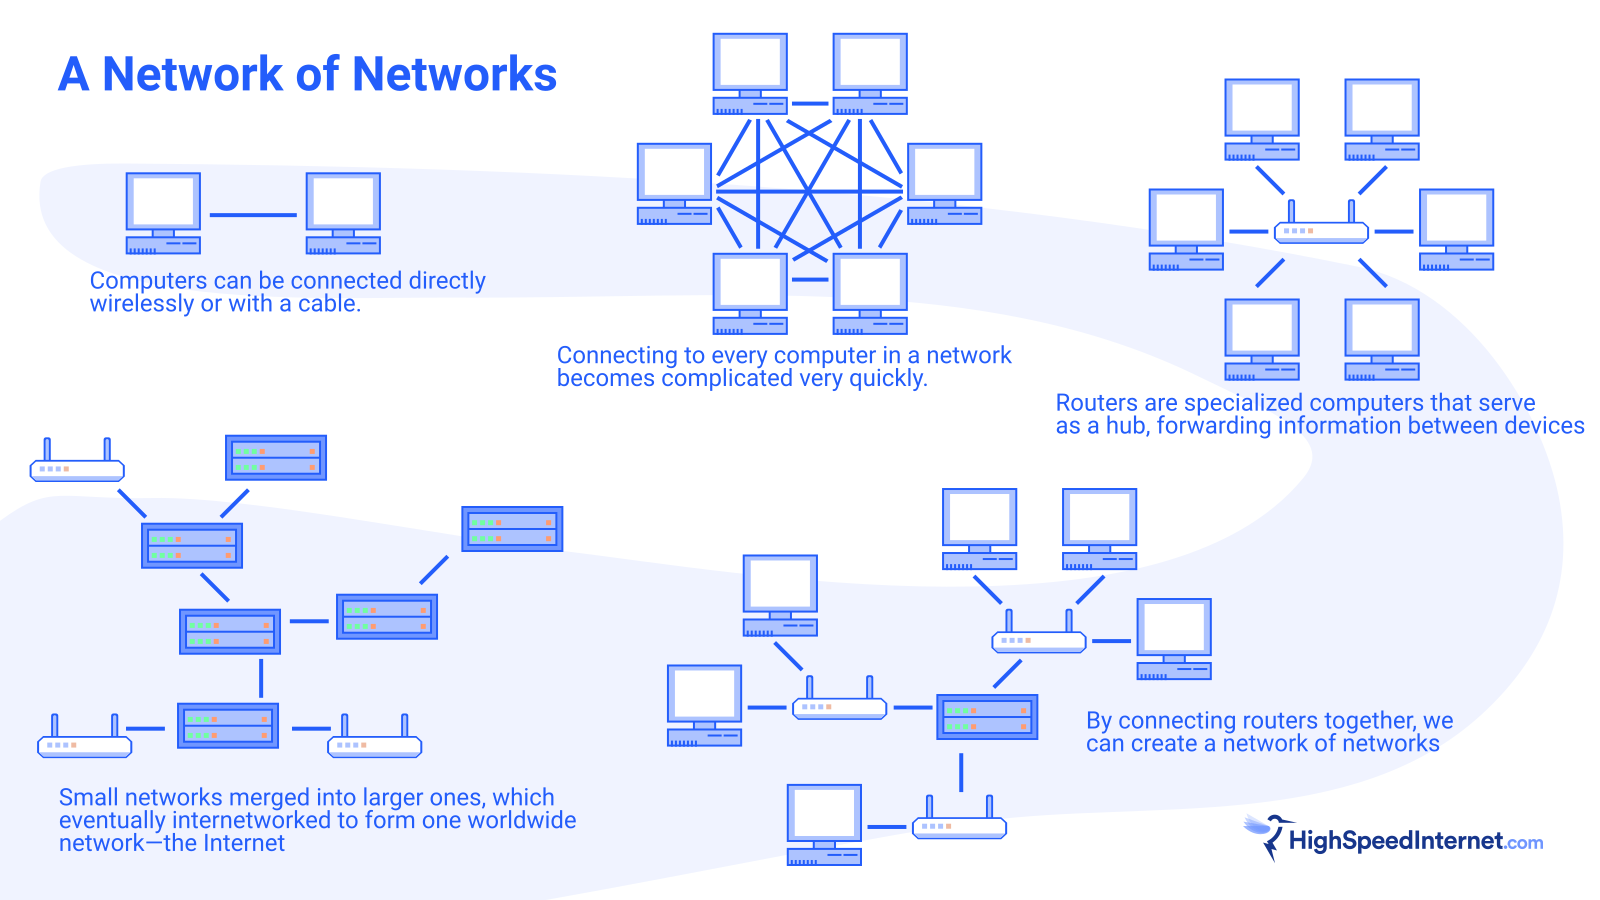
\includegraphics{networks}
\caption{Types of Networks}
\labfig{networks}
\end{marginfigure}

If the end goal is to connect computers with each other,
one naive solution might be to connect all the computers
with each other. Although this might seem intuitive at
first, this quickly gets out of hand when the number of
computers keep increasing.

If we have $n$ computers, then the number of connections
required to connect all the computers with each other
is given by the formula

\[
\frac{n(n-1)}{2} = \frac{n^2 - n}{2}
\]

This is a quadratic function and grows very quickly.

\begin{marginfigure}
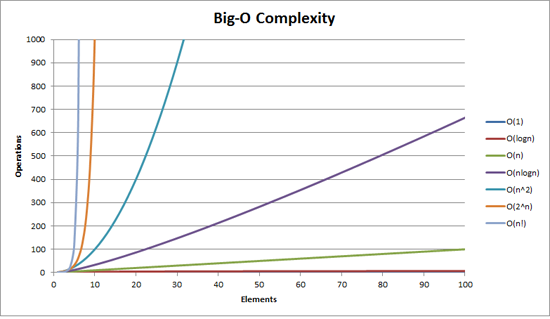
\includegraphics{complexity}
\caption{Growth Rate of Different Functions - Note how quickly $n^2$ grows}
\labfig{complexity}
\end{marginfigure}

This means it will cost a lot to connect all the computers
to each other. This is applicable not only in computer
networking with physical wires, but in many other fields.
Take an examples of airlines and airplane routes. If there
were $n$ airports, then the number of routes required to
connect all the airports is given by the same formula.
This would be disastrous for the economy and the environment
if we ran so many airplanes daily. So what gives?

\textbf{Hub and Spoke Network}

\begin{marginfigure}
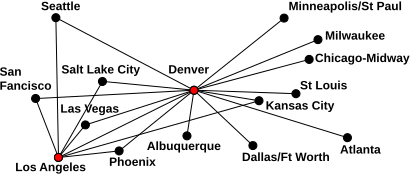
\includegraphics{airlines}
\caption{Hub and Spoke Model Employed by Airlines}
\labfig{airlines}
\end{marginfigure}

The solution to this problem is to use a hub and spoke
model, where there are one, or multiple, central hubs
which connect to many other nodes. Any path from any
node to another goes through one or more hubs. This
reduces the number of connections required to connect
all the nodes.

This is the solution used in airlines, and also in
most computer networks.
\sidenote{
  Although computer networks use a hub model
  for the local area network, the network of
  networks, especially the gateway routers
  follow a mesh model to ensure redundancy
  and make the network more robust.
}

Due to this, networks can be classified into three
broad categories based on their geographical area
coverage.

\begin{marginfigure}
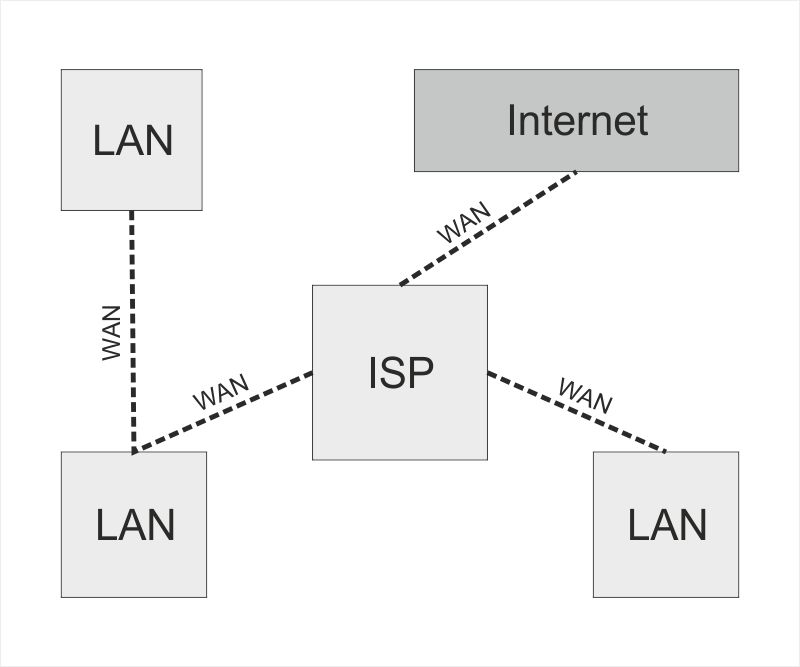
\includegraphics{wan}
\caption{LAN and WAN connecting to the Internet}
\labfig{wan}
\end{marginfigure}

\begin{itemize}
\item \textbf{Local Area Network (LAN)}: A network
that covers a small geographical area, like a
home, office, or a building.
\item \textbf{Metropolitan Area Network (MAN)}:
A network that covers a larger geographical area,
like a city or a town.
\item \textbf{Wide Area Network (WAN)}: A network
that covers a large geographical area, like a
country or the entire world.
\end{itemize}

To connect these networks to computers and also
to each other, we require some special devices.

\subsection{Devices in a Network}

In computer networks, this hub of the
Hub and Spoke Model can either be a
level 1 hub, a level 2 switch, or a level 3 router.

\textbf{Hub}

A hub will simply broadcast the message to all
the connected nodes. This causes a lot of traffic
to be generated and is not very efficient. Hub does
not have the capability to identify which node
is who. This is called a level 1 hub.
\sidenote{
  To understand more about the levels, refer
  \href{https://en.wikipedia.org/wiki/OSI\_model}{OSI Model}
}

\textbf{Switch}

A switch is smarter than a hub. It can identify
each device connected to it and can send the
packets of data only to the intended recipient.
This is more efficient than a hub. This is called
a level 2 switch since it uses the level 2 of the
OSI model (Data Link Layer) to identify the devices.
This means that the devices are identified by their
MAC addresses.
Using this, you can only communicate with devices
in your local network. This is useful for a home
network or a office network. But we cannot communicate
with the entire world using this, since it doesn't
understand IP addresses.

\textbf{Router}

\begin{marginfigure}
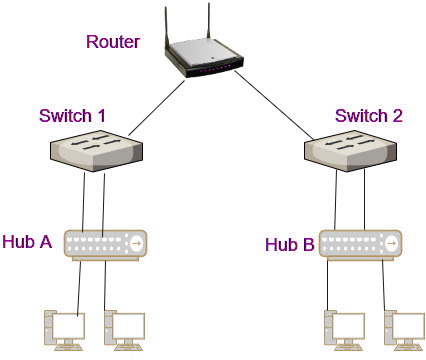
\includegraphics{hsr}
\caption{Hub, Switch, Router connecting to the Internet}
\labfig{hsr}
\end{marginfigure}

A router is even smarter than a switch. It can
understand IP addresses and can route the packets
from one network to another. This is called a level 3
router since it uses the level 3 of the OSI model
(Network Layer) to identify the devices. This means
that the networks are identified by their IP addresses.
This is what we use to connect to the internet.
The internet is nothing but a whole lot of routers
communicating with each other to find the optimal
path to send the packets to its destination.
Border Gateway Protocol (BGP) is the protocol used
by routers to communicate with each other and find
the optimal path. They usually are connected in a
mesh network to ensure redundancy and robustness.

\textbf{Level 3 Switch}

A level 3 switch, or a routing switch, is a switch
with the capabilities of a router. It can understand
the language of IP addresses and can route the packets
to different networks. This is useful in large
organizations where there are many networks and
each network can be divided into subnetworks called
VLANs.

\marginnote{
  You can read more about the differences between
  these devices
  \href{https://www.cbtnuggets.com/blog/technology/networking/l1-l2-vs-l3-whats-the-difference}{online}.
}

So, in short, internet is a network of network
of \dots networks. It is a hierarchical structure
connecting all the computers in the world.
Some computers are connected earlier in the
hierarchy (usually the ones closer geographically)
and some are connected later.

\subsection{IP Addresses}

So how do routers know which where to send the
data packets? This is where IP addresses come in.
To communicate over the internet, two computers
need to know their public IP addresses. The routers
then finds the optimal path to send the data packets
to the destination network.

IP addresses are of two types: IPv4 and IPv6.
The most common one is IPv4, which is a 32-bit
address represented as four octets separated by
dots. For example,

\[
162.136.73.21
\]

Here, each octet can take values from 0 to 255.
\sidenote{
  An octet is a group of 8 bits. Since an IP
  address is 32 bits, it is represented as 4
  groups of 8 bits.
  8 bits can only represent numbers from 0 to 255.
  since $2^8 = 256$.
}
Technically all such combinations are possible
IP addresses, resulting in
$2^{32} = 4,294,967,296$ possible IP addresses.
That is a lot of IP addresses, but not enough
for the growing number of devices in the world.

This is where IPv6 comes in. IPv6 is a 128-bit
address represented as 8 groups of 4 hexadecimal
digits separated by colons. For example,

\[
2001:0db8:85a3:0000:0000:8a2e:0370:7334
\]

\marginnote{
  Notice that there are some groups of zeros
  in the address. These can be compressed by
  writing only one zero in place of multiple
  zeros in each group. Further, any leading
  zeros can be omitted for each group.
  Making the above address as
  \lstinline|2001:db8:85a3:0:0:8a2e:370:7334|.
  Further, if there are multiple groups of zeros,
  they can be compressed to \lstinline|::|.
  This can be used only once in an address.
  Doing this, the above address can be compressed
  further to
  \lstinline|2001:db8:85a3::8a2e:370:7334|.
}

This results in
\[
  2^{128} = 340282366920938463463374607431768211456
\]
possible IP addresses, which is a lot more than
IPv4.

\subsection{Subnetting}

\textbf{Legacy Classes}

\[
10.125.42.62 \rightarrow 0 0 0 0 1 0 1 0 . 0 1 1 1 1 1 0 1 . 0 0 1 0 1 0 1 0 . 0 0 1 1 1 1 1 0
\]

Recall that an IP address, although represented as
four octets, is actually a 32-bit address. This
means that in binary form, an IP address is a
string of 32 1s and 0s. Using the first four bits,
we can classify an IP address into five classes.

\begin{itemize}
\item \textbf{Class A}: The first bit is `0`. The
IP addresses in the range 0.0.0.0 to 127.255.255.255.
\item \textbf{Class B}: The first two bits are `10`.
IP addresses in the range 128.0.0.0 to 191.255.255.255.
\item \textbf{Class C}: The first three bits are `110`.
IP addresses in the range 192.0.0.0 to 223.255.255.255.
\item \textbf{Class D}: The first four bits are `1110`.
IP addresses in the range 224.0.0.0 to 239.255.255.255.
These are reserved for multicast addresses.
\item \textbf{Class E}: The first four bits are `1111`.
IP addresses in the range 240.0.0.0 to 255.255.255.255.
These are reserved for experimental purposes.
\end{itemize}

However, these classes do not simply assign an IP to
each machine. They are further divided into the
network part and the host part.

Class A assigns the first octet to the network part,
this is used to identify which network the machine
is in. The remaining three octets are used to identify
the host in that network. This means that a class A
network can have $2^{24} - 2 = 16,777,214$ hosts.
However, there can only be $2^{7} = 128$ class A
networks. Thus, class A networks are used by large
organizations which have many hosts, but not many
large organizations exist, so 128 networks are enough.

Similarly, class B assigns the first two octets to
identify the network and the remaining two octets
to identify the host. This means that a class B
network can have $2^{16} - 2 = 65,534$ hosts.
And there can be $2^{14} = 16,384$ class B networks.
These are used by medium-sized organizations, which
are plenty in number, and have a moderate number of
hosts.

The same goes for class C networks, where the first
three octets are used to identify the network and
the last octet is used to identify the host. This
network can have $2^{8} - 2 = 254$ hosts. And there
can be $2^{21} = 2,097,152$ class C networks. These
are used by small organizations, which are plenty
in number, and have a small number of hosts.

\textbf{Subnet Masks}

\begin{definition}[Subnetting]
The process of dividing a network into smaller network
sections is called subnetting.
\end{definition}

Usually, each network has only one subnet, which
contains all the hosts in that network. However,
the network can be further divided into smaller
subnetworks, each containing a subset of the hosts.
This is useful in large organizations where the
network is divided into departments, and each
department is given a subnetwork.

To indicate which part of the IP address is the
network part and which part is the host part, we
use a subnet mask. A subnet mask is a 32-bit
number where the first $n$ bits are 1s and the
remaining bits are 0s. The number of 1s in the
subnet mask indicates the number of bits used
to identify the network. For example, for the
IP Address \lstinline|192.168.0.15|, it can be
written in binary as
\[
1100 0000 - 1010 1000 - 0000 0000 - 0000 1111
\]

As we know, it belongs to the class C network,
where the first three octets are used to identify
the network, and the rest is used to identify the
host. So the default network mask is

\[
1111 1111 - 1111 1111 - 1111 1111 - 0000 0000
\]

or \lstinline|255.255.255.0| in decimal.
The network portion of the IP address is
found by taking the bitwise AND
\sidenote{
  The bitwise AND operation is a binary operation
  that takes two equal-length binary representations
  and performs the logical AND operation on each pair
  of corresponding bits. The result in each position
  is 1 if the first bit is 1 and the second bit is 1;
  otherwise, the result is 0.
}
of the IP address and the subnet mask.
This results in the network address
\[
1100 0000 - 1010 1000 - 0000 0000 - 0000 0000
\]
which is \lstinline|192.168.0.0| and the host address
is \lstinline|0000 1111| which is $15$.

However, if we do not require all the 8 bits in the
host space
\sidenote{
  That is, if we have less than 254 hosts in the
  network.
}
then we can use some of the initial bits of the
host space to identify subnetworks. This is called
subnetting.

For example, the netmask of \lstinline|255.255.255.0|
leaves 8 bits for the host space, or $2^8 - 2 = 254$
\sidenote{
  We subtract 2 from the total number of hosts
  to account for the network address and the
  broadcast address, which are the first(0)
  and the last(255) addresses in the network.
}
hosts. If we want to split this network into
two subnets, we can use the MSB of the host space
for representing the subnetworks. This results in
each subnet having $2^7 - 2 = 126$ hosts.

\begin{remark}
Observe that we effectively lost two available addresses
from the total number of hosts in the network.
Earlier we could have $254$ hosts, but now we can
have only $126 \times 2 = 252$ hosts. This is because
each subnet also reserves the first and the last
address for the network address and the broadcast
address.
\end{remark}

To do this, we change the subnet mask to
\[
1111 1111 - 1111 1111 - 1111 1111 - 1000 0000
\]
which can be represented as \lstinline|255.255.255.128|.

This gives us two subnets, one with the address range
of \lstinline|192.168.0.1| to \lstinline|192.168.0.127|, and
another of \lstinline|192.168.0.129| to \lstinline|192.168.0.255|.

\subsection{Private and Public IP Addresses}

But what if we want to communicate with computers
in our local network? This is where private IP
comes in. Some ranges of IP addresses are reserved
for private networks. These are not routable over
the internet. Each LAN has a private IP address
range, and the router translates these private
addresses to the public IP address when sending
the packets over the internet. The assignment
of these private IP addresses is done by the
DHCP server
\sidenote{
  Dynamic Host Configuration Protocol (DHCP) is
  a network management protocol used on Internet
  Protocol networks whereby a DHCP server dynamically
  assigns an IP address and other network configuration
  parameters to each device on a network so they can
  communicate with other IP networks.
}
in the router.

Each class of networks has a range of IP addresses
that are reserved for private networks.

\begin{table*}[h!]
\caption{Private IP Address Ranges}
\labtab{privateip}
\begin{tabular}{c c c c}
\toprule
Class & Network Bits & Address Range & Number of Addresses \\
\midrule
\textbf{Class A} & 8 & \lstinline|10.0.0.0| - \lstinline|10.255.255.255| & 16,777,216 \\
\textbf{Class B} & 12 & \lstinline|172.16.0.0| - \lstinline|172.31.255.255| & 1,048,576 \\
\textbf{Class C} & 16 & \lstinline|192.168.0.0| - \lstinline|192.168.255.255| & 65,536 \\
\bottomrule
\end{tabular}
\end{table*}

\subsection{CIDR}

However, this practice of subdividing IP addresses
into classes is a legacy concept, and not followed
anymore. Instead, we use CIDR (Classless Inter-Domain
Routing) to announce how many bits are used to identify
the network and how many bits are used to identify the
host.

For example, we could express the idea that the IP address
\lstinline|192.168.0.15| is associated with the netmask
\lstinline|255.255.255.0| by using the CIDR notation of
\lstinline|192.168.0.15/24|. This means that the first
$24$ bits of the IP address given are considered
significant for the network routing.

This is helpful because not all organizations fit
into the tight categorization of the legacy classes.

\subsection{Ports}

Ports usually refer to physical holes in a computer
where you can connect a cable. However, in networking,
ports refer to logical endpoints for communication.

\begin{definition}[Port]
A port or port number is a number assigned to uniquely identify
a connection endpoint and to direct data to a specific service.
At the software level, within an operating system, a port is a
logical construct that identifies a specific process or a type
of network service.
\end{definition}

For any communication between two computers, the data
needs to be sent to a specific port. This is because
there are multiple services running on a computer, and
the operating system needs to know which service to
direct the data to.

There are $2^{16} = 65,536$ ports available for use.
However, the first $1024$ ports are reserved for
well-known services. These are called the \textbf{well-known
ports} and are used by services like HTTP, FTP, SSH, etc.
The well known ports can be found in \reftab{wellknownports}.

Other ports, from $1024$ to $49151$, are registered ports,
these ports can be registered with the Internet Assigned
Numbers Authority (IANA) by anyone who wants to use them
for a specific service.

Ports from $49152$ to $65535$ are dynamic ports, these
are used by the operating system for temporary connections
and are not registered.

Whenever you send a request to a web server for example,
the request is sent to the server's IP address and the
port number \lstinline|80| which is the default port for
HTTP
\sidenote{
  or \lstinline|443| for HTTPS.
}
but the port number from your (the client) side is
usually a random port number from the dynamic port range.
This is a short-lived port number and is used to
establish a connection with the server.

These kinds of ports which are short-lived and used
to establish a connection are called \textbf{ephemeral ports}.

\begin{table*}[h!]
\caption{Well-known Ports}
\labtab{wellknownports}
\begin{tabular}{c l c}
\toprule
Port Number & Service & Protocol \\
\midrule
20 & File Transfer Protocol (FTP) Data Transfer & TCP \\
21 & File Transfer Protocol (FTP) Command Control & TCP \\
22 & Secure Shell (SSH) Secure Login & TCP \\
23 & Telnet remote login service& TCP \\
25 & Simple Mail Transfer Protocol (SMTP)& TCP \\
53 & Domain Name System (DNS) service & TCP/UDP \\
67, 68 & Dynamic Host Configuration Protocol (DHCP) & UDP \\
80 & Hypertext Transfer Protocol (HTTP) & TCP \\
110 & Post Office Protocol (POP3) & TCP \\
119 & Network News Transfer Protocol (NNTP) & TCP \\
123 & Network Time Protocol (NTP) & UDP \\
143 & Internet Message Access Protocol (IMAP) & TCP \\
161 & Simple Network Management Protocol (SNMP) & UDP \\
194 & Internet Relay Chat (IRC) & TCP \\
443 & HTTP Secure (HTTPS) HTTP over TLS/SSL & TCP \\
546, 547 & DHCPv6 IPv6 version of DHCP & UDP \\
\bottomrule
\end{tabular}
\end{table*}

\subsection{Protocols}

\begin{definition}[Protocols]
In computing, a protocol is a set of rules that define
how data is transmitted between devices in a network.
\end{definition}

There are many protocols used in networking, some of
the most common ones are

\begin{itemize}
    \item \textbf{HTTP}: HyperText Transfer Protocol
    \item \textbf{HTTPS}: HyperText Transfer Protocol Secure
    \item \textbf{FTP}: File Transfer Protocol
    \item \textbf{SSH}: Secure Shell
    \item \textbf{SMTP}: Simple Mail Transfer Protocol
    \item \textbf{POP3}: Post Office Protocol
    \item \textbf{IMAP}: Internet Message Access Protocol
    \item \textbf{DNS}: Domain Name System
    \item \textbf{DHCP}: Dynamic Host Configuration Protocol
    \item \textbf{NTP}: Network Time Protocol
    \item \textbf{SNMP}: Simple Network Management Protocol
    \item \textbf{IRC}: Internet Relay Chat
    \item \textbf{BGP}: Border Gateway Protocol
    \item \textbf{TCP}: Transmission Control Protocol
    \item \textbf{UDP}: User Datagram Protocol
\end{itemize}

These protocols act on the different layers of the
OSI model. For example, HTTP, HTTPS, FTP, SSH, etc.
are application layer protocols, while TCP, UDP, etc.
are transport layer protocols.

\subsection{Firewalls}

\begin{definition}[Firewall]
  A firewall is a network security system that monitors
  and controls incoming and outgoing network traffic
  based on predetermined security rules.
\end{definition}

A fireewall acts as a barrier between your computer
and the internet. It monitors the incoming and outgoing
traffic and blocks any traffic that does not meet the
security rules. This is useful to prevent unauthorized
access to your computer and to prevent malware from
entering your computer and/or communicating with the
outside world.

\begin{lstlisting}[language=bash]
$ sudo ufw enable # Enable the firewall
$ sudo ufw allow 22 # Allow SSH
$ sudo ufw allow 80 # Allow HTTP
$ sudo ufw allow 443 # Allow HTTPS
$ sudo ufw status # Check the status of the firewall
\end{lstlisting}

\subsection{SELinux}

We can have additional security by using SELinux
in addition to the firewall. SELinux is a security
module that provides access control security policies.
SELinux is short for Security-Enhanced Linux.
It provides a flexible Mandatory Access Control (MAC)
that restricts the access of users and processes to
files and directories.

\textbf{Least Privilege Principle}

\begin{definition}[Least Privilege Principle]
The principle of least privilege (POLP) is an important
concept in computer security, promoting minimal user
profile privileges on computers based on users' job
necessity.
\end{definition}

This principle states that a user should have only
the minimum privileges required to perform their job.
This principle is applied throughout linux, and also
in SELinux.

You can check if \textbf{SELinux} is enabled by running

\begin{lstlisting}[language=bash]
$ sestatus
\end{lstlisting}

If SELinux is enabled, you can check the context of
a file or a directory using

\begin{lstlisting}[language=bash]
$ ls -lZ
\end{lstlisting}

However, if SELinux is not enabled, it will show
a \lstinline|?| in the context.

If SELinux is enabled, you can set the context of a
file or a directory using the \lstinline|chcon| command.

\textbf{RBAC Items}

\begin{definition}[Role-Based Access Control (RBAC)]
Role-Based Access Control (RBAC) is a policy-neutral
access control mechanism defined around roles and
privileges. The components of RBAC such as role-permissions,
user-role, and role-role relationships make it simple
to perform user assignments.
\end{definition}

SELinux uses the concept of RBAC to control the access
of users and processes to files and directories.

There are four components in the SELinux context
that are used to control the access of users and
processes to files and directories, as shown in
\reffig{selinux}.

\begin{figure}[h!]
  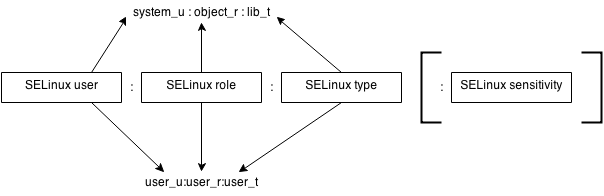
\includegraphics{selinux}
  \caption{SELinux Context}
  \labfig{selinux}
\end{figure}

\begin{itemize}
  \item \textbf{User}: The user who is trying to access
    the file or directory.
  \item \textbf{Role}: The role of the user, which defines
    the permissions of the user.
  \item \textbf{Type}: The type of the file or directory.
  \item \textbf{Domain}: The domain
    \sidenote{or type or sensitivity}
    of the process trying to access the file or directory.
\end{itemize}

\textbf{Modes of SELinux}

\begin{itemize}
  \item \textbf{Enforcing}: In this mode, SELinux is enabled
    and actively enforcing the security policies.
  \item \textbf{Permissive}: In this mode, SELinux is enabled
    but not enforcing the security policies. It logs the
    violations but does not block them.
  \item \textbf{Disabled}: In this mode, SELinux is disabled
    and not enforcing any security policies.
\end{itemize}

You can change the mode of SELinux by editing the
\lstinline|/etc/selinux/config| file.

\begin{lstlisting}[language=bash]
$ sudo vim /etc/selinux/config
\end{lstlisting}

\textbf{Tools for SELinux}

\begin{itemize}
  \item \textbf{sestatus}: Check the status of SELinux.
  \item \textbf{semamange}: Manage the SELinux policy.
  \item \textbf{restorecon}: Restore the context of files
    and directories.
\end{itemize}


\subsection{Network Tools}

There are a lot of tools in GNU/Linux used for managing,
configuring, and troubleshooting networks. Some of the
important tools are listed in \reftab{networktools}.

\begin{table*}[h!]
  \caption{Network Tools}
  \labtab{networktools}
  \begin{tabular}{c l}
    \toprule
    \textbf{Tool} & \textbf{Description} \\
    \midrule
    \lstinline|ip| & Show / manipulate routing, devices, policy routing and tunnels \\
    \lstinline|ping| & To see if the remote machine is up \\
    \lstinline|traceroute| & Diagnostics the hop timings to the remote machine \\
    \lstinline|nslookup| & Ask for conversion of IP address to name \\
    \lstinline|dig| & DNS lookup utility \\
    \lstinline|netstat| & Print network connections \\
    \href{https://mxtoolbox.com/}{mxtoolbox} & Public accessibility of your server \\
    \href{https://whois.com/}{whois} & Information about the domain \\
    \lstinline|nmap| & Network port scanner \\
    \lstinline|wireshark| & Network protocol analyzer and packet sniffer \\
    \bottomrule
  \end{tabular}
\end{table*}

\textbf{ip}

To find out the private IP address of the NICs of your system,
you can run the \lstinline|ip addr| command.
\sidenote{
  \lstinline|ip a| also works.
}

\begin{lstlisting}[language=bash]
$ ip addr
1: lo: <LOOPBACK,UP,LOWER_UP> mtu 65536 qdisc noqueue state UNKNOWN group default qlen 1000
    link/loopback 00:00:00:00:00:00 brd 00:00:00:00:00:00
    inet 127.0.0.1/8 scope host lo
       valid_lft forever preferred_lft forever
    inet6 ::1/128 scope host noprefixroute
       valid_lft forever preferred_lft forever
2: eno1: <BROADCAST,MULTICAST,UP,LOWER_UP> mtu 1500 qdisc fq_codel state UP group default qlen 1000
    link/ether 1c:1b:0d:e1:5d:61 brd ff:ff:ff:ff:ff:ff
    altname enp3s0
    inet 192.168.0.109/24 brd 192.168.0.255 scope global dynamic eno1
       valid_lft 7046sec preferred_lft 7046sec
    inet6 fe80::68e2:97e0:38ec:4abc/64 scope link noprefixroute
       valid_lft forever preferred_lft forever
\end{lstlisting}

Here you can see there are two interfaces, \lstinline|lo|
and \lstinline|eno1|. The \lstinline|lo| interface is the
loopback interface, and the \lstinline|eno1| interface
is the actual network interface. The IP address of
the \textbf{lo} interface is usually always \lstinline|127.0.0.1|.
This address is used to refer to the same system in terms
of IP address without knowing the actual private IP of
the system in the LAN.

The IP address of the \textbf{eno1} interface is the
private IP address allocated by your router. This is
not your public IP address, which is the address of
your router on the internet. Usually public IPs are
statically assigned by ISPs and are not changed often.
It is configured in your router.

Private IPs however often needs to be assigned dynamically
since devices can connect and disconnect from the network
at any time. This is done by the DHCP server in your router.

\begin{remark}
The NIC name can be different in different systems.
For a ethernet connection, it is usually \lstinline|eno1|
or \lstinline|eth0| which is the legacy name. For a wifi
NIC, it is usually \lstinline|wlan0|.
\end{remark}

\begin{remark}
  Earlier the tool used to check the network status
  was \lstinline|ifconfig|. However, this tool is deprecated
  now and should not be used. The new tool to check the
  network status is \lstinline|ip|.
\end{remark}

\textbf{ping}

The \lstinline|ping| command is used to check if a remote
server is up and running. It sends an \textbf{ICMP}
\sidenote{
  Internet Control Message Protocol (ICMP) is a
  supporting protocol in the Internet protocol suite.
  It is used by network devices, including routers,
  to send error messages and operational information
  indicating success or failure when communicating
  with another IP address.
}
packet to the remote server and waits for a response.

\begin{remark}
  Only a positive response from the server indicates
  that the server is up and running. A negative response
  does not necessarily mean that the server is down.
  Servers can be configured to not respond to ICMP packets.
\end{remark}

\begin{lstlisting}[language=bash]
$ ping -c 4 google.com # Send 4 ICMP packets to google.com
PING google.com (172.217.163.206) 56(84) bytes of data.
64 bytes from maa05s06-in-f14.1e100.net (172.217.163.206): icmp_seq=1 ttl=114 time=45.6 ms
64 bytes from maa05s06-in-f14.1e100.net (172.217.163.206): icmp_seq=2 ttl=114 time=45.4 ms
64 bytes from maa05s06-in-f14.1e100.net (172.217.163.206): icmp_seq=3 ttl=114 time=45.3 ms
64 bytes from maa05s06-in-f14.1e100.net (172.217.163.206): icmp_seq=4 ttl=114 time=45.8 ms

--- google.com ping statistics ---
4 packets transmitted, 4 received, 0% packet loss, time 3004ms
rtt min/avg/max/mdev = 45.316/45.524/45.791/0.181 ms
\end{lstlisting}

The response of the \lstinline|ping| command shows the
time taken for the packet to reach the server and
also the resolved IP address of the server.

\textbf{nslookup}

Another tool to lookup the associated IP address of
a domain name is the \lstinline|nslookup| command.

\begin{lstlisting}[language=bash]
$ nslookup google.com
Server:         192.168.0.1
Address:        192.168.0.1#53

Non-authoritative answer:
Name:   google.com
Address: 172.217.163.206
Name:   google.com
Address: 2404:6800:4007:810::200e
\end{lstlisting}

Here you can see the resolved IP address of the domain
is \lstinline|172.217.163.206|. If you copy this IP address
and paste it in your browser, you can see that the
website of google opens up.
The second address returned is the IPv6 IP Address.

The first lines mentioning the \textbf{Server}
is the \textbf{DNS Server} which returned the
resolution of the IP address from the queried
domain name.

\begin{remark}
  Notice that the DNS Server mentioned in the above
  output is actually a private IP. This is the IP
  address of the router in the LAN which acts as
  the DNS Server cache. However if you type the
  domain of a website which you have not visited,
  or have visited long ago into \lstinline|nslookup|,
  then the DNS Server mentioned will be the public
  address of the DNS Server, which might be your
  ISP's DNS Server, or some other public DNS Server.
\end{remark}

You can also use \textbf{mxtoolbox} to check the
IP address of your server from the public internet.

\textbf{dig}

Another tool to lookup the associated IP address of
a domain name is the \lstinline|dig| command.
It can also reverse lookup the IP address to find
the associated domain name.

\begin{lstlisting}[language=bash]
$ dig google.com

; <<>> DiG 9.18.27 <<>> google.com
;; global options: +cmd
;; Got answer:
;; ->>HEADER<<- opcode: QUERY, status: NOERROR, id: 31350
;; flags: qr rd ra; QUERY: 1, ANSWER: 1, AUTHORITY: 4, ADDITIONAL: 9

;; OPT PSEUDOSECTION:
; EDNS: version: 0, flags:; udp: 4096
; COOKIE: 3e5ff6a57c0fe2b3b5ce91b3666ae859ec9b6471261cecef (good)
;; QUESTION SECTION:
;google.com.			IN	A

;; ANSWER SECTION:
google.com.		50	IN	A	172.217.163.206

;; AUTHORITY SECTION:
google.com.		162911	IN	NS	ns1.google.com.
google.com.		162911	IN	NS	ns3.google.com.
google.com.		162911	IN	NS	ns4.google.com.
google.com.		162911	IN	NS	ns2.google.com.

;; ADDITIONAL SECTION:
ns2.google.com.		163913	IN	A	216.239.34.10
ns4.google.com.		163913	IN	A	216.239.38.10
ns3.google.com.		337398	IN	A	216.239.36.10
ns1.google.com.		340398	IN	A	216.239.32.10
ns2.google.com.		163913	IN	AAAA	2001:4860:4802:34::a
ns4.google.com.		163913	IN	AAAA	2001:4860:4802:38::a
ns3.google.com.		2787	IN	AAAA	2001:4860:4802:36::a
ns1.google.com.		158183	IN	AAAA	2001:4860:4802:32::a

;; Query time: 3 msec
;; SERVER: 192.168.0.1#53(192.168.0.1) (UDP)
;; WHEN: Thu Jun 13 18:18:52 IST 2024
;; MSG SIZE  rcvd: 331
\end{lstlisting}

And we can then feed the IP address to dig again, to find
the domain name associated with the IP address.

\begin{lstlisting}[language=bash]
$ dig -x 172.217.163.206

; <<>> DiG 9.18.27 <<>> -x 172.217.163.206
;; global options: +cmd
;; Got answer:
;; ->>HEADER<<- opcode: QUERY, status: NOERROR, id: 15781
;; flags: qr rd ra; QUERY: 1, ANSWER: 1, AUTHORITY: 4, ADDITIONAL: 9

;; OPT PSEUDOSECTION:
; EDNS: version: 0, flags:; udp: 4096
; COOKIE: 78a3c6e4e4b103f501380f62666ae89b3a3b52e8be388fe0 (good)
;; QUESTION SECTION:
;206.163.217.172.in-addr.arpa.	IN	PTR

;; ANSWER SECTION:
206.163.217.172.in-addr.arpa. 83966 IN	PTR	maa05s06-in-f14.1e100.net.

;; AUTHORITY SECTION:
217.172.in-addr.arpa.	78207	IN	NS	ns4.google.com.
217.172.in-addr.arpa.	78207	IN	NS	ns2.google.com.
217.172.in-addr.arpa.	78207	IN	NS	ns1.google.com.
217.172.in-addr.arpa.	78207	IN	NS	ns3.google.com.

;; ADDITIONAL SECTION:
ns1.google.com.		340332	IN	A	216.239.32.10
ns2.google.com.		163847	IN	A	216.239.34.10
ns3.google.com.		337332	IN	A	216.239.36.10
ns4.google.com.		163847	IN	A	216.239.38.10
ns1.google.com.		158117	IN	AAAA	2001:4860:4802:32::a
ns2.google.com.		163847	IN	AAAA	2001:4860:4802:34::a
ns3.google.com.		2721	IN	AAAA	2001:4860:4802:36::a
ns4.google.com.		163847	IN	AAAA	2001:4860:4802:38::a

;; Query time: 3 msec
;; SERVER: 192.168.0.1#53(192.168.0.1) (UDP)
;; WHEN: Thu Jun 13 18:19:58 IST 2024
;; MSG SIZE  rcvd: 382
\end{lstlisting}

Note that the answer we got after running
\href{https://google.com}{google.com} through
\textbf{dig} and then through \textbf{dig -x}
(maa05s06-in-f14.1e100.net) is
different from the original domain name.

This is because the domain name is resolved to
an IP address, and then the IP address is resolved
to a different domain name. This is because the
the domain name is actually an alias to the
cannonical name.

\begin{remark}
  The IP address you would get by running
  \textbf{dig} or \textbf{nslookup} on google
  would be different from the IP address you
  get when using \href{https://mxtoolbox.com/}{mxtoolbox}.
  This is because google is a large company and
  they have multiple servers which are load balanced.
  So someone in India might get a different IP address
  compared to someone in the US.
\end{remark}

To get the output of \lstinline|dig| in a more readable
and concise format, you can use the \lstinline|+short|
or \lstinline|+noall| option.

\begin{lstlisting}[language=bash]
$ dig +noall +answer google.com
google.com.		244	IN	A	172.217.163.206
\end{lstlisting}

\textbf{netstat}

The \lstinline|netstat| command is used to print network
connections, routing tables, interface statistics,
masquerade connections, and multicast memberships.

It is useful to find what connections are open on
your system, and what ports are being used by which
applications.

\begin{lstlisting}[language=bash]
$ netstat | head
Active Internet connections (w/o servers)
Proto Recv-Q Send-Q Local Address           Foreign Address         State
tcp        0      0 rex:53584               24.224.186.35.bc.:https TIME_WAIT
tcp        0      0 rex:56602               24.224.186.35.bc.:https TIME_WAIT
tcp        0      0 localhost:5037          localhost:43267         TIME_WAIT
tcp        0      0 localhost:5037          localhost:46497         TIME_WAIT
tcp        0      0 rex:35198               24.224.186.35.bc.:https TIME_WAIT
tcp        0      0 rex:44302               24.224.186.35.bc.:https TIME_WAIT
tcp        0      0 localhost:5037          localhost:55529         TIME_WAIT
tcp        0      0 localhost:5037          localhost:38005         TIME_WAIT
\end{lstlisting}


\vfill
\pagebreak
\section{SSH}
\subsection{What is SSH?}

The Secure Shell (SSH) Protocol is a protocol for secure
communication between two computers over a compromised
or untrusted network.
\sidenote{
  like the internet.
}
SSH uses encryption and authentication to secure the
communication between the two computers.

SSH is now the ubiquitous protocol for secure remote
access to servers, and is used by system administrators
all over the world to manage their servers.

SSH lets a user of a computer to log into the computer
from another computer over the network, to execute
any command in the terminal that they have access to.

SSH can also be used to transfer files between two
computers using the \lstinline|scp| command.

\subsection{History}

It was initially developed by Tatu Ylönen in
1995 as a replacement for the insecure Telnet and FTP
protocols when he found that someone had installed a
packet sniffer on the server of his university.

There are multiple implementations of the SSH protocol,
the most popular being OpenSSH, developed by the OpenBSD
project.
This is the implementation that is used in most of the
linux distributions as well.

\subsection{How does SSH work?}

\begin{marginfigure}
  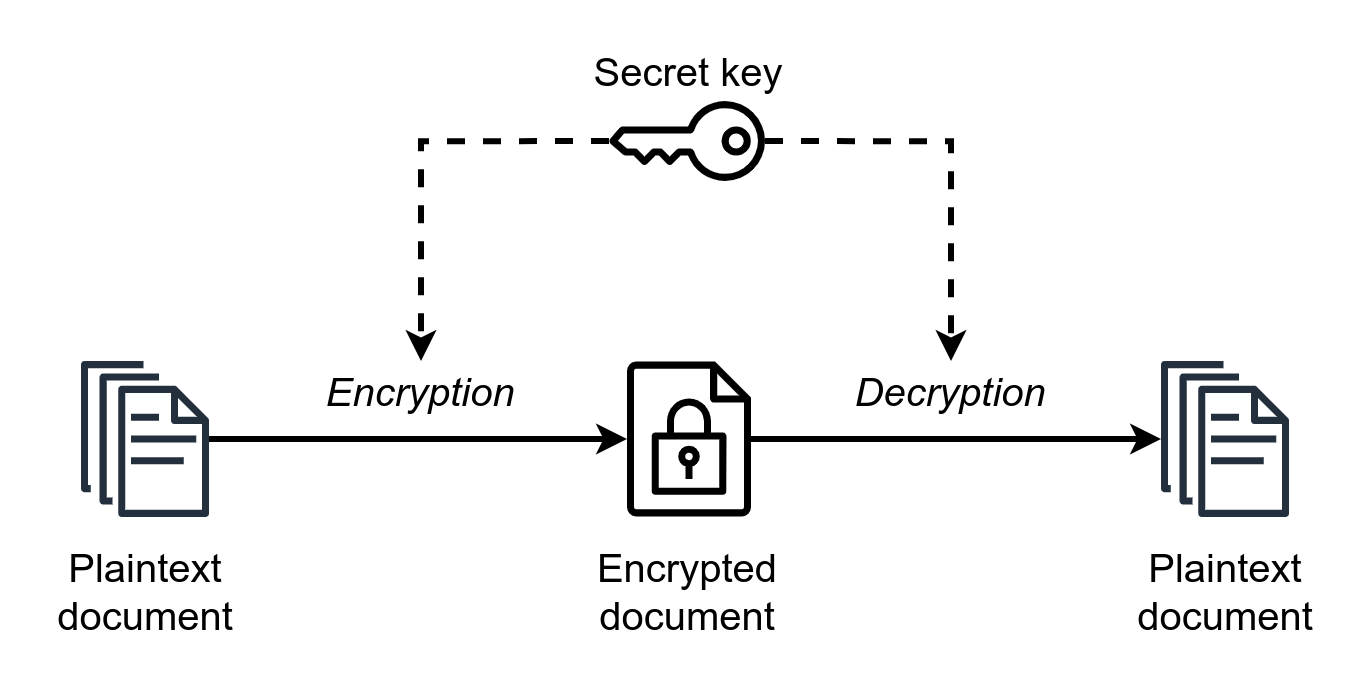
\includegraphics{sym-enc}
  \caption{Symmetric Encryption}
  \labfig{symenc}
\end{marginfigure}

SSH works by using symmetric and asymmetric encryption.
The data packets sent over the network are enctypted,
usually using AES symmetric encryption.
This ensures that even if the data packets are intercepted
by a man-in-the-middle attacker, they cannot be read
since they are encrypted.

To login into a remote server, all you need to do is
provide the username and the IP address or the domain
name of the server to the \lstinline|ssh| command.

\begin{marginfigure}
  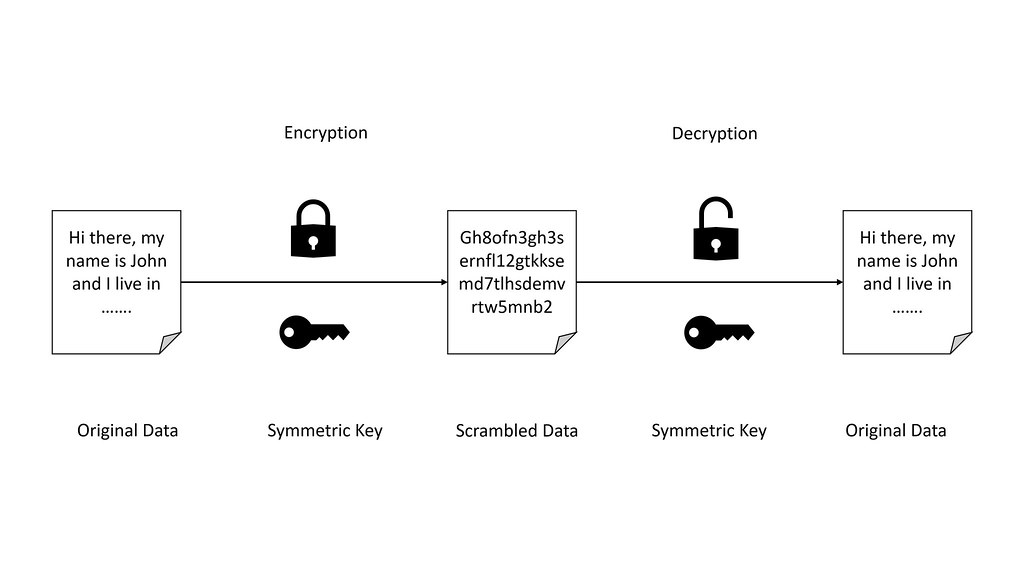
\includegraphics{encrypt}
  \caption{Symmetric Encryption}
  \labfig{encrypt}
\end{marginfigure}

\begin{lstlisting}[language=bash]
$ ssh username@ipaddress
\end{lstlisting}

\[
  \text{OR}
\]

\begin{lstlisting}[language=bash]
$ ssh username@domainname
\end{lstlisting}

SSH allows user to login to a remote server using
their username and password, but this is not encouraged
since it lets the user to be vulnerable to brute-force
attacks.

Another way to authenticate is by using public-private
key pairs.

\subsection{Key-based Authentication}

\begin{marginfigure}
  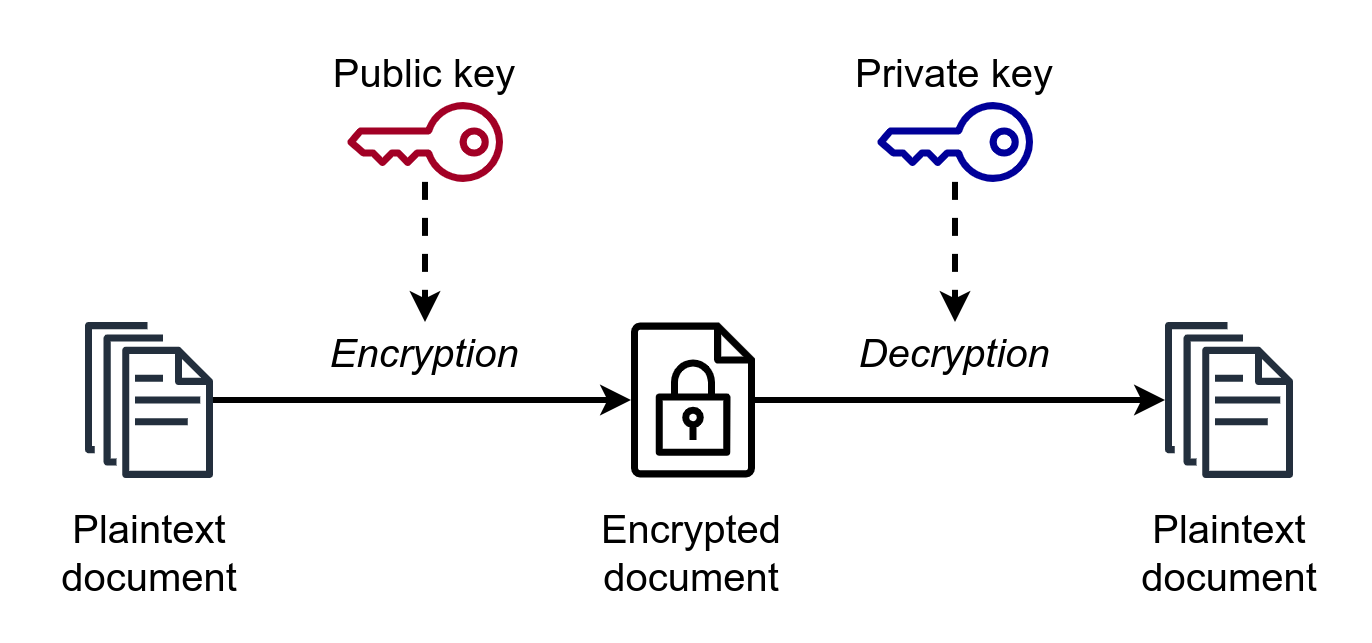
\includegraphics{ass-enc}
  \caption{Asymmetric Encryption}
  \labfig{ass-enc}
\end{marginfigure}

One of the most powerful features of SSH is its ability
to use public-private key pairs for authentication. In
our course, we emphasize the importance of this method.
Instead of relying on passwords, which can be vulnerable
to brute-force attacks, a pair of cryptographic keys is used.
The public key is stored on the server, while the private key
is kept secure on your local machine. This ensures a highly
secure and convenient way of accessing remote servers without
the need for constantly entering passwords.

\subsection{Configuring your SSH keys}

For this course, it is a must for you to not only
create, but also understand SSH keys.
Let us quickly see how to create a ssh key-pair
which can be used to login into a remote server.

We need to use the \lstinline|ssh-keygen|
command to create a new public-private
key pair.

\begin{lstlisting}[language=bash]
$ ssh-keygen
Generating public/private ed25519 key pair.
Enter file in which to save the key (/home/test1/.ssh/id_ed25519):
\end{lstlisting}

Here you have to either simply press enter to
continue with the default location, or you can
also type a custom location where you want to
save the key. If this is your first time creating
keys, it is recommended to use the default location.

\begin{remark}
  There are multiple algorithms that can be used
  to generate a key pair. The most common ones are
  RSA, DSA, and ED25519. The ED25519 algorithm is
  the new default algorithm used by OpenSSH since
  it is shorter yet more secure than RSA.
  If you have an outdated version of OpenSSH, you
  might get the default RSA algorithm.
  To change the algorithm, you can use the \lstinline|-t|
  flag along with the \lstinline|ssh-keygen| command.
  \begin{lstlisting}[language=bash]
  $ ssh-keygen -t rsa \end{lstlisting}
  will create a RSA key pair and using
  \begin{lstlisting}[language=bash]
  $ ssh-keygen -t ed25519 \end{lstlisting}
  will create a ED25519 key pair.
\end{remark}

Next, it will ask you to enter a passphrase.
You can enter a passphrase for added security,
or you can simply press enter to continue without
a passphrase. If you do add a passphrase, you will
have to always enter the passphrase whenever you
use the key. We can continue without a passphrase
for now by pressing enter.

\begin{lstlisting}[language=bash]
Enter passphrase (empty for no passphrase):
Enter same passphrase again:

Your identification has been saved in /home/username/.ssh/id_ed25519
Your public key has been saved in /home/username/.ssh/id_ed25519.pub
The key fingerprint is:
SHA256:n4ounQd6v9uWXAtMyyq7CdncMsh1Zuac5jesWXrndeA test1@rex
The key's randomart image is:
+--[ED25519 256]--+
|                 |
|                 |
|                 |
|          .      |
|      . S+ .  .  |
|   . *.O o=... . |
|    =o=o*+++ .E .|
|    o.=Bo*O o. . |
|     +**XB.+.    |
+----[SHA256]-----+
\end{lstlisting}

Our key pair has been generated. The private key
is stored in \lstinline|/home/username/.ssh/id\_ed25519|
and the public key is stored in
\lstinline|/home/username/.ssh/id\_ed25519.pub|.

Make sure to \textbf{never} share your private key with anyone.
Ideally, you dont even need to see the private key yourself.
You should only share the public key with the server
you want to login to.

\subsection{Sharing your public key}

\textbf{ssh-copy-id}

Finally, to share the public key with the server,
there are usually multiple ways. If the server
allows you to login using a password, you can
simply use the \lstinline|ssh-copy-id| command.
This command will take your username and password
to login to the server, and then copy the public
key which you provide to the server.

\begin{lstlisting}
$ ssh-copy-id -i /key/to/public/key username@ipaddress
\end{lstlisting}

\begin{remark}
  The \lstinline|-i| flag is used to specify the path
  to the public key. You can drop the \lstinline|.pub|
  from the path as well (making it the path to the
  private key), since \lstinline|ssh-copy-id| will
  automatically look for the public key.
  However, this flag is not required if you
  are using the default location.
  This is why using the default location is
  recommended for beginners.
  The simplified syntax then becomes
  \begin{lstlisting}[language=bash]
  $ ssh-copy-id username@ipaddress \end{lstlisting}
  The same applies for logging into the server
  using the \lstinline|ssh| command.
\end{remark}

\textbf{manual install}

However, most servers do not allow password login
at all, since it defeats the purpose of using
a public-private key pair. In such cases, you
need to somehow copy the public key to the server.

If you have physical access to the server, you
can simply copy the public key to the server
in the \lstinline|~/.ssh/authorized\_keys| file
of the server.

\begin{lstlisting}[language=bash]
$ file ~/someoneskey.pub
~/someoneskey.pub: OpenSSH ED25519 public key
$ cat ~/someoneskey.pub >> ~/.ssh/authorized_keys
\end{lstlisting}

\begin{remark}
  Make sure to use the \lstinline|>>| operator and
  not the \lstinline|>| operator. The \lstinline|>>|
  operator appends the contents of the file to
  the end of the file, while the \lstinline|>|
  operator overwrites the file, we do not want that.
\end{remark}

\textbf{System Commands Course}

However, in case of our course, you do not have access
to the server as well. To submit your \textbf{public key},
you have to login into the website
\url{https://se2001.ds.study.iitm.ac.in/passwordless}
using your institute credentials, and then submit
your public key in the form provided.

You can print out the contents of the public key
using the \lstinline|cat| command and copy the contents
into the form.

\begin{lstlisting}[language=bash]
[test1@rex ~]$ cat .ssh/id_ed25519.pub
ssh-ed25519 AAAAC3NzaC1lZDI1NTE5AAAAIDxh5EuvzQkGvsqlMQW3rOkY+wyo+2d6Y5CSqNGlLs2a test1@rex
\end{lstlisting}

You should copy the entire contents of the file, including
your username and hostname.

\subsection{How to login to a remote server}

You can then login into the server using the \lstinline|ssh|
command.

\begin{lstlisting}[language=bash]
$ ssh rollnumber@se2001.ds.study.iitm.ac.in
\end{lstlisting}

\[
  \text{OR, if not using the default location of key}
\]

\begin{lstlisting}[language=bash]
$ ssh -i /path/to/private/key rollnumber@se2001.ds.study.iitm.ac.in
\end{lstlisting}

If successful, you will be logged into the server
and the prompt will change to the server's prompt.

\begin{lstlisting}[language=bash]
[test1@rex ~]$ ssh 29f1001234@se2001.ds.study.iitm.ac.in
Last login: Mon Jun  3 07:43:22 2024 from 192.168.2.3
29f1001234@se2001:~$
\end{lstlisting}

Notice that the prompt has changed from \lstinline|test1@rex|
which was the prompt of your local machine, to
\lstinline|rollnumber@se2001| which is the prompt of the
server.

\subsection{Call an exorcist, there's a daemon in my computer}

What is \lstinline|sshd|?
It is a daemon.

\begin{definition}[Daemon]
  In multitasking computer operating systems, a daemon
  is a computer program that runs as a background process,
  rather than being under the direct control of an
  interactive user.
\end{definition}

There are many daemons running in your computer.
You can use \lstinline|systemctl status| to see the
loaded and active daemons in your computer.

\begin{lstlisting}[language=bash]
$ systemctl status
* rex
    State: running
    Units: 419 loaded (incl. loaded aliases)
     Jobs: 0 queued
   Failed: 0 units
    Since: Thu 2024-06-13 12:55:42 IST; 7h ago
  systemd: 255.6-1-arch
   CGroup: /
           |-init.scope
           | `-1 /usr/lib/systemd/systemd --switched-root --system --deserialize=43
           |-system.slice
           | |-NetworkManager.service
           | | `-547 /usr/bin/NetworkManager --no-daemon
           | |-adb.service
           | | `-558 adb -L tcp:5037 fork-server server --reply-fd 4
           | |-avahi-daemon.service
           | | |-550 "avahi-daemon: running [rex.local]"
           | | `-557 "avahi-daemon: chroot helper"
           | |-cronie.service
           | | `-621 /usr/sbin/crond -n
           | |-cups.service
           | | `-629 /usr/bin/cupsd -l
           | |-dbus-broker.service
           | | |-545 /usr/bin/dbus-broker-launch --scope system --audit
\end{lstlisting}

Here you can see some of the important daemons running,
such as \lstinline|NetworkManager| which is used to manage
the network connections, \lstinline|cronie| which is used
to run scheduled tasks, \lstinline|cups| which is used to
manage printers, etc.

\textbf{sshd}

sshd is the daemon that runs on the server and listens
to any incoming SSH connections. It is the daemon that
lets you login into the server using the SSH protocol.

Your own system might not be running the \lstinline|sshd|
daemon, since you are not running a server. However,
you can check if the \lstinline|sshd| daemon is running
using the \lstinline|systemctl| command.

\begin{lstlisting}[language=bash]
$ systemctl status sshd
* sshd.service - OpenSSH Daemon
     Loaded: loaded (/usr/lib/systemd/system/sshd.service; disabled; preset: disabled)
     Active: inactive (dead)
\end{lstlisting}

Here you can see that the \lstinline|sshd| daemon is
currently inactive. This is because I am not running
a server and don't usually login remotely to my
system. However, the output of the same command
would be something like as shown below
if it is enabled on your system.


\begin{lstlisting}[language=bash]
$ systemctl status sshd
* sshd.service - OpenSSH Daemon
     Loaded: loaded (/usr/lib/systemd/system/sshd.service; disabled; preset: disabled)
     Active: active (running) since Thu 2024-06-13 19:48:44 IST; 12min ago
   Main PID: 3583344 (sshd)
      Tasks: 1 (limit: 9287)
     Memory: 2.1M (peak: 2.3M)
        CPU: 8ms
     CGroup: /system.slice/sshd.service
             `-3583344 "sshd: /usr/bin/sshd -D [listener] 0 of 10-100 startups"

Jun 13 19:48:44 rex systemd[1]: Started OpenSSH Daemon.
Jun 13 19:48:45 rex sshd[3583344]: Server listening on 0.0.0.0 port 22.
Jun 13 19:48:45 rex sshd[3583344]: Server listening on :: port 22.
\end{lstlisting}

If we run the same command on the server, we can see
that it is running. However, we wont be able to
read the logs of the server, since we are not
authorized.


\marginnote{
  I have set the \lstinline|LC\_ALL| environment variable
  to the locale C while generating the
  above outputs to prevent latex errors.
  Ideally if you run the command, you will see
  a prettier unicode output.
}
\begin{lstlisting}
$ ssh username@se2001.ds.study.iitm.ac.in
username@se2001:~$ systemctl status sshd
* ssh.service - OpenBSD Secure Shell server
     Loaded: loaded (/lib/systemd/system/ssh.service; enabled; vendor preset: enabled)
     Active: active (running) since Thu 2024-06-13 12:32:47 UTC; 1h 57min ago
       Docs: man:sshd(8)
             man:sshd_config(5)
    Process: 732 ExecStartPre=/usr/sbin/sshd -t (code=exited, status=0/SUCCESS)
   Main PID: 745 (sshd)
      Tasks: 1 (limit: 4557)
     Memory: 22.0M
        CPU: 8.769s
     CGroup: /system.slice/ssh.service
             `-745 "sshd: /usr/sbin/sshd -D [listener] 0 of 10-100 startups"

Warning: some journal files were not opened due to insufficient permissions.
\end{lstlisting}

\begin{remark}
  Notice that there are some differences in the output
  when run from my local system and from the system
  commands server. Such as, the name of the service
  is \lstinline|ssh| on the server, while it is \lstinline|sshd|
  on my local system. Also the full name is \textbf{OpenBSD
  Secure Shell server} on the server, while it is
  \lstinline|OpenSSH Daemon| on my local system.
  The path of the service file is also different.
  This is because the server is running a ubuntu
  distribution whereas my local system runs an arch
  distribution. They have different packages for
  ssh, and hence the differences.
\end{remark}

\subsection{SCP}

\textbf{scp} is a command used to copy files between
remote servers.
It uses the \lstinline|ssh| protocol to copy files
in an encrypted manner over the network.

The syntax of the \lstinline|scp| command is similar
to the \lstinline|cp| command.

\begin{lstlisting}[language=bash]
$ scp username@ipaddress:/path/to/file /path/to/destination
\end{lstlisting}

This will copy a file from the remote server to your
local machine.

\begin{lstlisting}[language=bash]
$ scp /path/to/file username@ipaddress:/path/to/destination
\end{lstlisting}

This will copy a file from your local machine to the
remote server.
